% REV00 Tue 20 Jul 2021 08:12:01 WIB
% START Tue 20 Jul 2021 08:12:01 WIB

\chapter{Tigabelas}

% 11
\begin{figure}[htbp]
% h: here, where the figure appears in the text (use can always just use [h] )
% t: top,  top of the current page.
% b: bottom of the current page.
% p: page, top of the next available float space (sometimes end up being the end of the document).
\centerline{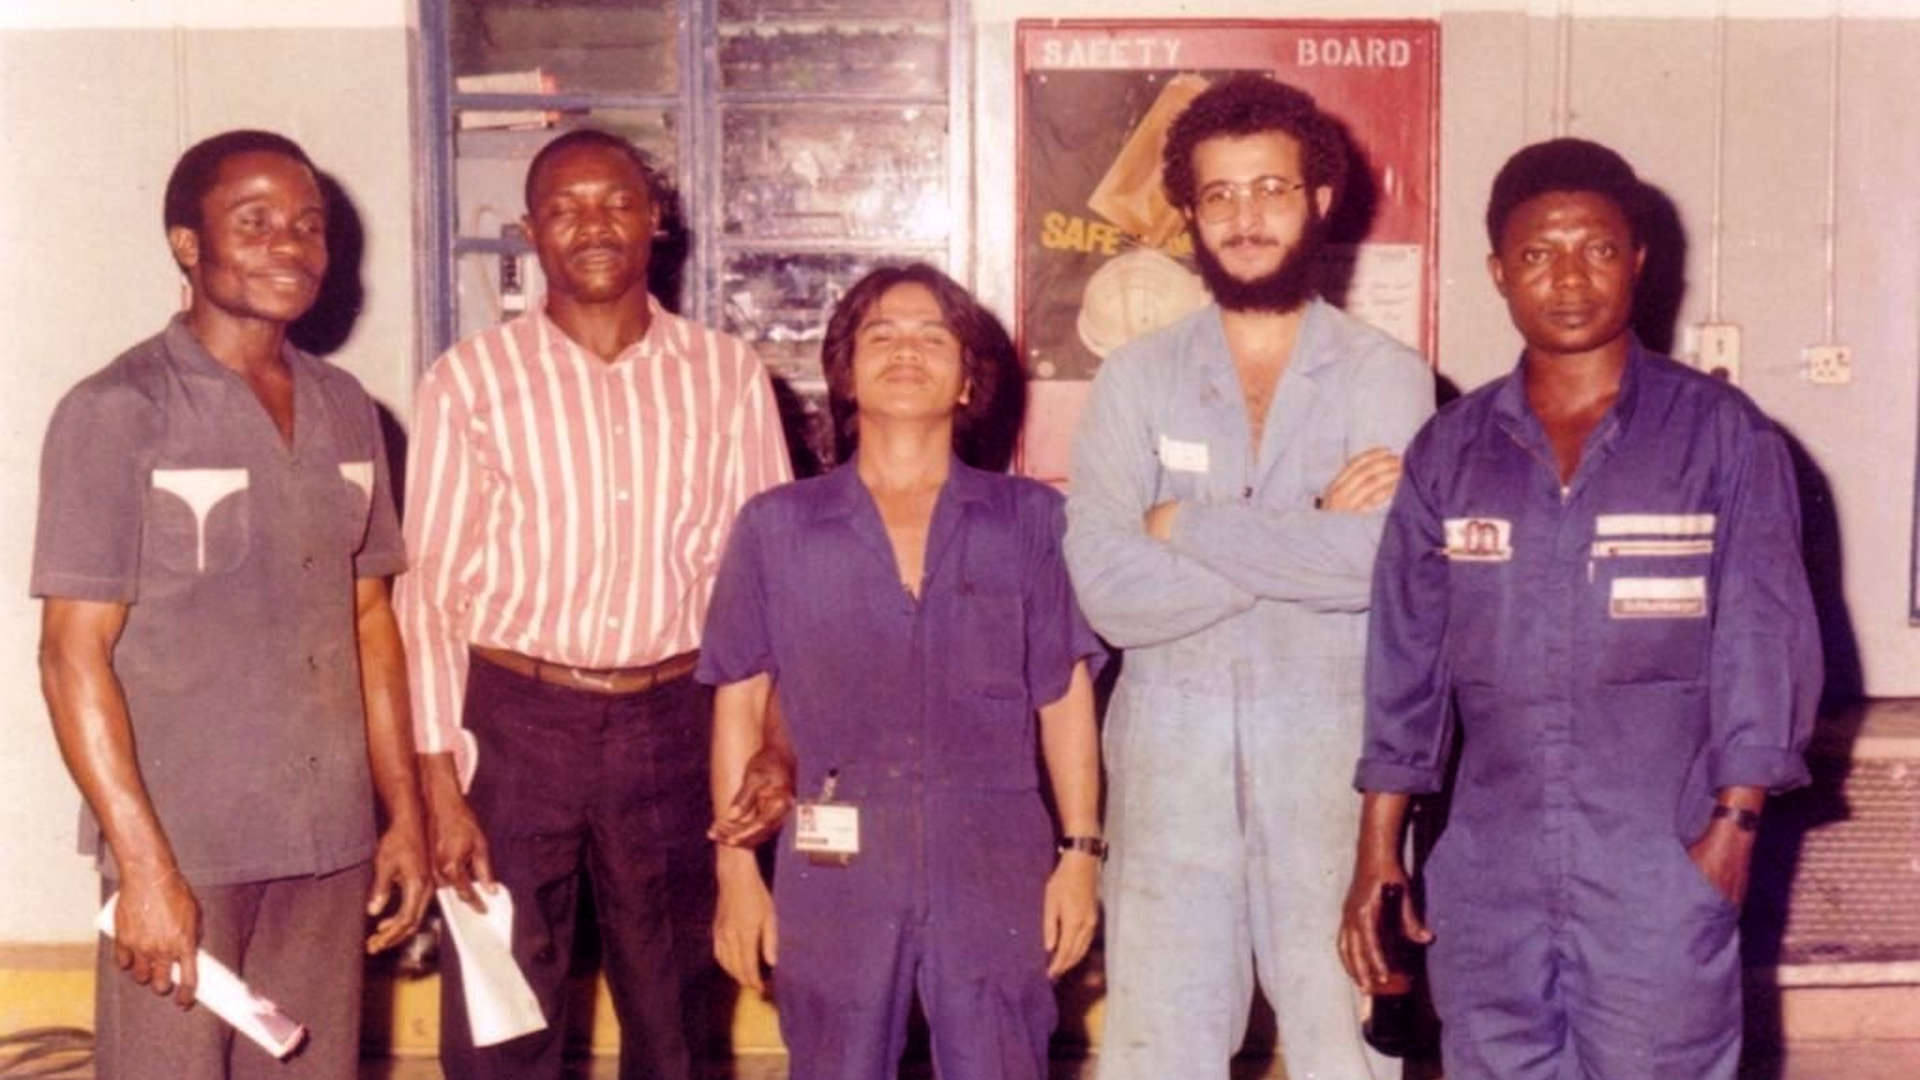
\includegraphics[scale=1.0]{01-13-01}}
\caption{"The Crazy Satiri of Schlumberger Nigeria" Sumber: Koleksi Kelvy Safira dan Fitria Clara Zora}
\label{01-13-01}
\end{figure}
%
Perjalanan pulang ke Jakarta terasa sangat lama. Dan memang jauh dari Port Harcourt, Nigeria ke Rawa Belong, Indonesia. Apalagi kalau menanggung kerinduan.

Daftar belanjanya sudah panjang: Beli rumah di Bintaro Puspita, beli baby benz boxer, dan ajak jalan-jalan orang tua dan anak istri ke Singapura, Jepang, dan California – lengkap dengan LA, Grand Canyon hingga San Diego.

(Semua terbayar dengan masa pelatihan dan kerja setahun di Nigeria. Kalau jadi dosen di UB kapan sampainya?)

Anda bayangkanlah berbagai keseruan baba dan ibunda “ii” jalan-jalan di negara antah berantah itu.

“Kok enggak ada TVRI ya?” tanya ibundanya. Lepas jam 10 malam TV malah menyiarkan hal-hal yang ‘bukan-bukan’, bukan main...

“Astaghfirullah…” ucap Babanya, sambil tutup mata sebelah. Sebentar saja. Ganti saluran. Sama juga! Matikan.

“Ini hari ini, pokoknya gua mau makan gado-gado,” pinta babanya.

Walaupun jalan-jalan itu menyenangkan, tetap rumah sendiri itu nomor satu. Buat Satiri, salah satu yang paling bikin kangen untuk pulang adalah, apalagi kalau bukan balas dendam untuk makan sayur asem dan ikan asin. Masakan pavorit keluarga, walaupun sekarang ditambah empal dan ayam goreng.

Saya sendiri sangat beruntung dulu sekali sempat mencicipi "sayur masak asem" buatan ibunda 'ii'. Ini sejenis sayur asem betawi, dengan sedikit rada pedas tanpa diberi gula, dan bumbunya terlebih dahulu dimasak dengan kunyit, sehingga kuahnya berwarna kuning.

Rasanya? Ni’meh! (beyond delicious; sugema kata orang Sunda)…

Lidah, mata dan hati kita akan dibuat tenang, cool, and nothing to be worried of.

Pada liburan pertamanya setelah training di Australia, yang paling diutamakannya adalah mengunjungi guru-gurunya: Bang Ipul, Pak Paijo, Pak Lesilolo, dan Jenderal O. Dia tidak pernah melupakan mereka.

Semua ia kunjungi satu per satu bersama semua anak-istrinya dan dengan buah tangan yang serba mewah. Pulang dari rumah mereka, ia merasa bahwa semua upayanya itu tidak sepadan dengan binar-binar kebahagiaan di mata mereka.

Ia bertekad untuk berbuat lebih banyak!

Satiri juga tidak pernah dapat melupakan perbuatannya memanfaatkan kuitansi tukang sayur dan cap himpunan mahasiswa (Himafi). Bagaimana aku harus membalasnya?

Baiklah. Ia meminta bantuan adik lelakinya yang pertama, Syahrul, untuk mengadakan wisata ke Bandung bagi siapa saja warga Jl. Salam, Rawa Belong, yang mau ikut. Wisata dua hari satu malam ke Lembang, Tangkuban Perahu dan mampir ke ITB. Gratis.

Apa yang terjadi? Terkumpul sekitar 200 orang dewasa dan anak-anak yang mau ikut berwisata.

“Bagaimana ini bang, banyak betul yang mau ikut?” tanya Syahrul kepada abangnya.

“Lu telpon Blue Bird, sewa 5 bus, dan pesan 100 kamar di Hotel Panghegar yah?”

“Panghegar? Ntu kan hotel paling mahal di Bandung?”

“Biarin ajah. Duitnya ada…”

(Saya terus terang sangat dekat dengan Syahrul. Berbeda dengan Satiri yang very high profile, Syahrul itu sangat polos dan jujur, mahasiswa IKJ dan guru kesenian di SMP. Kami berdua tidak pernah bosan mendiskusikan tentang Seni dan Sastra. Sayang, dia sudah mendahului kita sekitar akhir 80an. Al Fatihah untuk Bang Syahrul...)

Nah, kebayang kan berapa dana yang ia habiskan? Tidak ada yang bisa membantah bahwa pada acara ini Satiri mau pamer. Tapi anda juga bisa memandangnya dengan cara yang berbeda. Dia ingin menunjukkan bahwa apapun bisa dilakukan oleh orang Betawi, sama dengan orang-orang lainnya, asalkan kita mau berusaha dan berpikir keras!

Selebihnya, mengajak orang kampung Rawa Belong melihat kampung orang itu juga bagus. Dan pastinya perjalanan itu inspiratif bagi anak-anak remaja.

Anda mau dan berani melakukan hal semacam itu?

Yang juga rada gila adalah kelakuannya pas mampir ke kampus pada liburan kali itu. Satiri dan keluarga tentu naik Mercedesnya. Yang lainnya cukuplah naik bus blue bird, bus wisata terbaik saat itu.

Baby benz boxer masuk ke parkiran kecil di samping Himafi, belakangnya Ruang 1201, Lab Bosscha yang legendaris itu. Pas Satiri keluar dari mobil, entah bagaimana keluarlah Pak Dosen S, yang terkenal paling “killer” dan rada-rada enggak jelas.

“Ini Satiri ya… Waah hebat kamu sudah jadi orang kaya ya?”

“Iya Pak, saya sudah jadi orang kaya..” katanya mantap seraya memamerkan jam Rolex hitamnya.

“Gara-gara Fismat Pak…!” Hahahah...

Itu pelajaran Fismat yang diampu Dosen S banyak menelan korban. Beberapa mahasiswa DO karena tidak lulus-lulus di pelajaran itu. Ada juga yang harus mengambilnya 5 kali untuk bisa sekedar lulus dapat nilai D. Naah…
.
.
***

Pas liburan tiga bulan! Satiri memboyong istri dan anaknya ke Nigeria.

Rumah kontrakan di Nigeria cukup besar dan sudah ada telfon. Ingat bahwa status Satiri di perusahaan adalah bujangan!

Jadi, kalau Satiri tidak di rumah. Telfon tidak boleh diangkat. Kalau Satiri yang menelfon? Ada kodenya: Telfon dibiarkan berdering tiga kali, langsung dimatikan, dan ditelfon kembali. Yah, kucing-kucingan… Itu hanya untuk menyaring telefon dari Shlumberger Eropa. Tetapi boss dan semua rekan kerjanya juga tahu dia sudah berkeluarga.

Pekerjaan wireline itu lama-lama membosankan buat Satiri. Tantangannya sekedar teknis printal-printil di lapangan. Tidak ada hal besar yang mencengangkan seperti waktu dia berkenalan dengan Fisika Statistik. Fenomena alam yang semuanya selama ini dianggap serba pasti, deterministik, koq dibahas pakai statistik?

Orang bisa jijingkrakan ketika di pelajaran ini paham arti delta Dirac, bahwa nol dikali bilangan tak hingga sama dengan satu! Ada sisir Dirac, ada boson, dan ada distribusi Bose-Einstein. Sedapnya…

Tapi wireline duitnya sedap jugalah…

Untuk menghilangkan kebosanan di kampung Fort Harcourt Nigeria itu, Satiri dan istrinya banyak bermain gitar menanyi bersama. Fitria pandai ngaji, ya pandai nyanyi jugalah. Lagu-lagu Dangdut maupun lagu-lagu Barat.

Akhirnya mereka menyanyi bersama di acara-acara family gathering perusahaan. Ditampilkan lagu dangdut berpasangan yang segera memukau semua orang. Lagu “Malam Terakhir”:

\begin{verbatim}
Malam ini malam terakhir bagi kita
Untuk mencurahkan rasa rindu di dada

Esok aku akan pergi lama kembali
Kuharapkan agar engkau sabar menanti
Esok aku akan pergi lama kembali
Kuharapkan agar engkau sabar menanti

Aku akan sabar menantimu kembali
Selamat jalan dan sampai berjumpa lagi

Esok kita akan berpisah
Tentu hari-hari 'kan jadi sunyi
Esok kita akan berpisah
Tentu hati akan rindu sekali

Semakin lama kita berpisah
Semakin mesra kita berjumpa

Malam ini malam terakhir bagi kita
Untuk mencurahkan rasa rindu di dada
Kita akan berjumpa di saat bahagia
Di saat malam pesta perkawinan kita

Mengapa, mengapa hatiku berdebar-debar. Seakan-akan ku ragu
Untuk merelakan kepergianmu, kasih
Mengapa, mengapa hatiku berkata-kata. Seakan-akan berbisik
Bahwa kita tidak akan berjumpa lagi

Kepergianku hanya untuk kembali
Kita berpisah untuk berjumpa lagi
\end{verbatim}
.
.
Yang enggak ngerti dangdut, yang enggak ngerti bahasa Indonesia, semua ikut berjoged Dangdut. Senaaang…

Satiri sudah memperkenalkan Dangdut kepada dunia.

Belakangan semua acara gathering Schlumberger ditunda jika Saitiri sedang tugas ke lapangan! Demikian juga dengan semua acara pertetanggaan.

(Beberapa hari lalu Fitria menyampaikan kepada saya bahwa di hari-hari sebelumnya beberapa keluarga Schlumberger Nigeria menghubunginya untuk menyampaikan belasungkawa dan menegaskan persaudaraan mereka)

Hidup itu, ya bagaimana kita menikmatinya dan untuk menjadi berarti.
.
.
***

Kerja wireline di Nigeria sudah nyaris empat tahun, bagaimanapun juga itu adalah tempat antah-berantah. Apa akal?

“Boss, lubang-lubang bor di Indonesia itu memanggil-manggil saya…” katanya membuka tawaran. Sekaligus ancaman.

Sementara orang lain dag-dig-dug apa kontraknya akan diperpanjang, dia malah bikin pre-emptive strike: Serangan dadakan sebelum musuh menyerang!

“Are you crazy or what?”

“It is my name. You know it...”

“Satiri, kemarin sore saya baru saja dapat berita dari Pusat bahwa kamu akan ditempatkan ke Argentina. Saya sedang mikir-mikir bagaimana akan menyampaikannya ke kamu...” kata bosnya separuh menyerah.

“Then, forget about it…”

Yang mereka berdua sama-sama tahu dan tidak membicarakannya adalah bahwa toko sebelah (Halliburton, Baker and Hughes, dll) juga beredar di Indonesia.

“Okay. Get out…” kata bossnya nyerah benaran.
\\[10pt]

Sumber tulisan asli \url{https://www.facebook.com/reno.alamsyah.94/posts/10226594469034023}

